%=========================================================================
% (c) Michal Bidlo, Bohuslav K�ena, 2008

%%%%%%%%%%%%%%%%%%%%%%%%%%%%%%%%%%%%%%%%%%%%%%%%%%%%%%%%%%%%%%%%%%%%%%%%%%%%%%%%
\chapter{Introduction} 
One of the essential metrics for measuring VoIP gateway's performance is the
number and quality of simultaneous calls. It is affected mostly by the
computational demands of used communication protocols and number of registered
users. While the count of registered users provides very limited room for 
improvement by the nature of the problem itself, there could be wide variety
of approaches in implementing the protocol stacks. 

The communication protocols for VoIP gateway can be divided into two groups. 
Signalization, which consists mostly of textually represented protocols, where 
the messages' occurrence is either periodical with quite small frequency, or 
based on the users initiative which is a stochastical event depending on the 
activity of the user. However, generally the recurrence of both is rather 
similar. Comparably more resources during indirect simultaneous call sessions 
consumes processing the second group of protocols, transport of multimedia 
packets. Since security has recently grown to be necessary feature in VoIP 
communication and the encryption and decryption processes are designed with the 
idea of optimization, it is primary scope of interest of this thesis.



Development and results in the areas of parallel architectures shows that many
procedures could be distinctively accelerated by executing the algorithm on the
processing unit capable of parallel computations. Therefore, target of this 
thesis is implementation and analysis of parallel processing of encrypted
real-time multimedia data transfer.



Chapter \ref{chapter:srtp} describes the structures and algorithms used in 
Secure Real-time Transport Protocol. Increased attention is devoted to 
explanation of Advanced Encryption Standard, which is default cipher used in 
SRTP, including brief theoretical background and analysis of SRTP and AES. 
Because SRTP doesn't provide key exchange mechanism for symmetric AES cipher, 
the chapter also includes description of selected protocol extensions for this
 task.

Chapter \ref{chapter:gpgpu} provides basic information about graphic processing 
unit and the usage of GPU for general purpose computations. Part of the chapter 
is principal explanation of OpenCL framework and its elementary usage for the 
developer. As the parallel processing is diverse and wide study, the area of 
parallel paradigm that could be associated to the further implementation of
this thesis is mentioned with particular interest and focus. 

Chapter \ref{chapter:design} defines the term SIP gateway for the context of 
this thesis, discusses the design of such gateway and includes
listing of selected further implemented protocol stacks, their mutual 
interaction and possible improvement of processing the passing data. The highest
amount of attention is devoted to the comparison of different approaches to
design of SRTP stack and identification of main characteristics of native
OpenCL programming pattern in contrast to persistent thread model. The advantages
of both parallel implementations over serial code executed on the same hardware
is mentioned as well. Short introduction and description of used design patterns
is included in order to provide better comprehensibility of the application 
schemes.

Chapter \ref{chapter:implementation} covers the reference implementation of
the previous theoretical part of this thesis, used techniques and algorithms and
reasoning behind their selection. Even though the focus of the thesis is
primarily research of available contemporary methods there were many
restrictions. The requirements of this chapter arise from currently used
implementation and hardware limitation of the gateway.

Finally chapters \ref{chapter:results} and \ref{chapter:conclusion} summarize
the potential benefits of usage the GPGPU for the number of maximal simultaneous 
calls and shows visualization of achieved results in improvement and decrease of
latency. Also these chapter discusses possible contribution to related topics, 
such as transcoding of media compressing codecs which parallel implementation 
may provide even higher level of improvement.









%%%%%%%%%%%%%%%%%%%%%%%%%%%%%%%%%%%%%%%%%%%%%%%%%%%%%%%%%%%%%%%%%%%%%%%%%%%%%%%%
\chapter{Secure Real-time Transport Protocol}\label{chapter:srtp}
To achieve confidentiality and necessary security for real-time multimedia
transmission over TCP/IP connection there has been invented SRTP\cite{
rfc3711}. Except previously mentioned, it provides message
authentication and replay protection for both RTP and RTCP traffic, 
however, the thesis is going to focus on the implementation and computation
time of the security. The default cipher is AES in counter mode.

\section{Packet Structure}
SRTP packet can be described as RTP extension. It keeps the RTP fields of
the packet such as:
\begin{itemize}
\item Version (V) -- two bit number which currently is equal to 2.
\item Padding (P) -- boolean value whether the padding is set.
\item Extension (X) -- if this field is set, fixed header must be followed by
exactly one extension header.
\item CSRC count (CC) -- number of CSRC identifiers that follow the fixed 
header.
\item Marker (M) -- interpretation defined by a profile.
\item Payload Type (PT) -- identifies the type of payload
\item Sequence Number (SEQ) -- increments by one for each RTP packet.
\item Timestamp (TS) -- reflecting the exact moment the payload was sampled.
\item Synchronization Source Identifier (SSRC) -- identifier of RTP 
synchronization source within the single RTP session.
\item Contributing Source Identifiers (CSRC) -- list of 0 to 15 items 
identifying contributing sources.
\end{itemize}

The SRTP protocol defines that only payload is encrypted and also describes new 
fields in the RTP header.

\begin{itemize}
\item Master Key Identifier (MKI) -- unique identifier of the master key 
(previously signaled) to be used in session key derivation.
\item Authentication Tag -- carries message authentication data. If both
encryption and authentication are used, encryption should be applied first.
\end{itemize}

The packet length is variable and depends on number of CSRC used and length
of payload. The following scheme describes the packet with proportional
sizes of each field.

\begin{figure}[H]
\centering
\begin{verbatim}
    0                   1                   2                   3
  0 1 2 3 4 5 6 7 8 9 0 1 2 3 4 5 6 7 8 9 0 1 2 3 4 5 6 7 8 9 0 1
  +-+-+-+-+-+-+-+-+-+-+-+-+-+-+-+-+-+-+-+-+-+-+-+-+-+-+-+-+-+-+-+-+<+
  |V=2|P|X|  CC   |M|     PT      |       sequence number         | |
  +-+-+-+-+-+-+-+-+-+-+-+-+-+-+-+-+-+-+-+-+-+-+-+-+-+-+-+-+-+-+-+-+ |
  |                           timestamp                           | |
  +-+-+-+-+-+-+-+-+-+-+-+-+-+-+-+-+-+-+-+-+-+-+-+-+-+-+-+-+-+-+-+-+ |
  |           synchronization source (SSRC) identifier            | |
  +=+=+=+=+=+=+=+=+=+=+=+=+=+=+=+=+=+=+=+=+=+=+=+=+=+=+=+=+=+=+=+=+ |
  |            contributing source (CSRC) identifiers             | |
  |                               ....                            | |
  +-+-+-+-+-+-+-+-+-+-+-+-+-+-+-+-+-+-+-+-+-+-+-+-+-+-+-+-+-+-+-+-+ |
  |                   RTP extension (OPTIONAL)                    | |
+>+-+-+-+-+-+-+-+-+-+-+-+-+-+-+-+-+-+-+-+-+-+-+-+-+-+-+-+-+-+-+-+-+ |
| |                          payload  ...                         | |
| |                               +-------------------------------+ |
| |                               | RTP padding   | RTP pad count | |
+>+-+-+-+-+-+-+-+-+-+-+-+-+-+-+-+-+-+-+-+-+-+-+-+-+-+-+-+-+-+-+-+-+<+
| ~                     SRTP MKI (OPTIONAL)                       ~ |
| +-+-+-+-+-+-+-+-+-+-+-+-+-+-+-+-+-+-+-+-+-+-+-+-+-+-+-+-+-+-+-+-+ |
| :                 authentication tag (RECOMMENDED)              : |
| +-+-+-+-+-+-+-+-+-+-+-+-+-+-+-+-+-+-+-+-+-+-+-+-+-+-+-+-+-+-+-+-+ |
|                                                                   |
+- Encrypted Portion*                      Authenticated Portion ---+
\end{verbatim}
\caption[SRTP packet structure]{SRTP packet structure.}
\end{figure}

\section{Cryptographic Context}
In order to implement SRTP stack in the application, it is necessary to
preserve certain information about each encrypted session, which is 
called \textit{cryptographic context}. It must consist of the following:

\begin{itemize}
\item Rollover Counter -- 32-bit unsigned number, records how many times 
has the RTP sequential number been reseted to zero passed the value 65~535.
\item Highest Received SEQ -- 16-bit unsigned number
\item Identifier of the Encryption Algorithm -- the cipher and its mode
\item Replay List -- containing indices of recently received and 
authenticated SRTP packets
\item MKI -- if the MKI is present in current session, the length
of the MKI field in octets, actual value of currently used MKI
\item Master Keys -- enumeration of random and secret master keys
and counter for each key of how many packets have been sent with
that key. Single Master Key identifies SRTP stream and corresponding SRTCP
stream.
\item Session Keys -- current key for encryption and authentication
including stored their lengths in \texttt{n\_e} and \texttt{n\_a}
\end{itemize}

And for every master key, the cryptographic context may contain also
random but possibly public \textit{Master Salt} which will be used in 
key derivation.

\section{Master Key Exchange}
There are three most common protocols for key exchange in SRTP session between 
the end users -- SDES, MIKEY, and ZRTP. They differ in what protocol in VoIP 
communication they extend, provided security guarantees and possible 
communication overhead.

\textbf{ZRTP} is a protocol extension of RTP for secure establishing session key 
using Diffie-Hellman key exchange improved for detection of man-in-the-middle 
attack, which is briefly described in section \ref{mitm}, \cite{rfc6189}.
Another advantage of the improvement is that it doesn't require any prior shared 
secret nor public key infrastructure.

\textbf{SDES} is protocol extension of SDP\cite{rfc:sdp, rfc:sdes} typically in 
SIP\cite{rfc:sip} message. It is responsibility of the SIP stack to protect the 
key as secured secret, which is possible via TLS connection for instance.

\textbf{MIKEY} defines the key exchange as part of SDP payload in SIP message.
The algorithm is basic Diffie-Hellman which requires either prior shared secret
or PKI\footnote{ Public Key Infrastructure for digital certificates}. The SIP 
stack doesn't have to protect the transferred information any further.



\section{Protocol Summary}
Main concerns about the use of SRTP are whether the increase of computational
complexity and packet size don't make RTP hardly usable and what degree of
security does it provide.

\subsubsection*{Computational Overhead}
In VoIP communication the time has essential impact on the quality of
transmitted information, therefore it is important that ensuring the 
security of RTP wouldn't increase the latency over the acceptable level.
Among common limitations of real-time communications 
belong\cite{perkins:rtp2003}:
\begin{itemize}
\item Maximal tolerable latency round-trip time 300ms.
\item Smaller packet loss than 5\%.
\item Sensitivity to factors that are difficult to objectively measure
such as jitter.
\end{itemize}

It has been proven that increase in size of the packet SRTP is
insignificant compared to the RTP\cite{srtp:analysis2, srtp:analysis1}.
Average throughput of secured VoIP is usually around 2\% more than 
unsecured VoIP.



\subsubsection*{Security}
VoIP suffers from many similar security threats as other standard internet
services. 

\textit{Man in the middle}\label{mitm} in computer security is form of active 
eavesdropping. The attacker creates connections to both endpoints of the session
which allows him to monitor, record or modify the packets in communication 
making the endpoints believe that the conversation is secured. 
Protection against such attack could be achieved by key negotiating protocol
\textit{ZRTP} which is able to detect this activity\cite{rfc6189}.

\textit{Denial of service} is considered an attempt to make target machine 
unavailable to to its intended users. Typical method of this attack is to 
saturate the target machine with excessive requests that could lead to 
overloading the machine. Replay protection mechanism of SRTP with replay lists 
and authentication headers provide sufficient protection against DoS 
attack\cite{rfc3711, cisco:srtp}.

%%%%%%%%%%%%%%%%%%%%%%%%%%%%%%%%%%%%%%%%%%%%%%%%%%%%%%%%%%%%%%%%%%%%%%%%%%%%%%%%
\section{AES}
This section treats necessary theoretical background of Advanced Encryption 
Standard, which is the default cipher, and as the text has been written the only
cipher, of Secure Real-time Transport Protocol used in VoIP communication.

\textit{Advanced Encryption Standard} is symmetric block cipher which means 
it uses the same key for both encryption and decryption and encodes the
input in uniform sized blocks. The algorithm was developed to supersede
\textit{Data Encryption Standard} due to various security reasons\footnote
{ For instance COPACOBANA is FPGA based machine that could find 
an exhaustive key for DES in no longer than a week\cite{copacobana}.} in 
electronic data transmission. 

For this purpose National Institute of Standards and Technology (NIST)
announced public competition for new encryption standard in 1997 and 
considering multiple requirements the \textit{Rijndael}\footnote{ Rijndael
was original name of the AES as abbreviation of authors' names -- Joan 
Daemen and Vincent Rijmen.} was selected as the most suitable algorithm
for the task\cite{AES-FIPS}. 

\subsection{Mathematical Preliminaries}
All the bytes in AES are interpreted as 8-bit values in finite field $2^8$.
For better readability the values are printed using hexadecimal notation.
Following mathematical therms and operations are used in AES algorithm:

\subsubsection*{Galois field}
In algebra Galois field is finite field with finite number of elements.
Common notation is $GF(p^k)$ where $p$ is prime number and $k$ is positive
natural number. Therefore it is possible to classify the Galois fields 
by their size, because only single $GF(p^k)$ exists for each $p$ and $k$.
Characteristics of the field is equal to the $p$.

Each byte is in fact a polynomial with degree equal to 7 with coefficients
$b_i$ 0 or 1 and this notation $b_7x^7 + b_6x^6 + b_5x^5 + b_4x^4 + b_3x^3
+ b_2x^2 + b_1x^1 + b_0$. The decimal number 95 could be represented as:
\begin{itemize}
\item $5F$ in hexadecimal
\item $0101~1111$ in binary as a byte
\item $x^6 + x^4 + x^3 + x^2 + x^1 + 1$ as polynomial with degree equal to 7
\end{itemize}

\subsubsection*{Addition}
Addition is defined as addition of coefficinets of both polynomials modulo
2. This operation has the same result as bitwise XOR and because 
each value is its own inversion, addition and substraction are equal
operations.

\subsubsection*{Multiplication}
Multiplication is defined as multiplication of both polynomials modulo
irreducible polynomial of degree eight. For AES the irreducible polynomial
is defined as
\begin{equation}
m(x) = x^8 + x^4 + x^3 + x + 1
\end{equation}

\subsubsection*{Multiplication by $x$}
Multiplication of binary polynomial by polynomial $x$ results in polynomial of
higher degree therefore the result must be reduced modulo $m(x)$. Following
equation is the binary polynomial multiplied by polynomial $x$.

\begin{equation}
b_7x^8+b_6x^7+b_5x^6+b_4x^5+b_3x^4+b_2x^3+b_1x^2+b_0x
\end{equation} 

If $b_7 = 1$ the result must be XORed with the polynomial $m(x)$. This operation
can be accomplished as bitwise left shift and XOR with $1B$.

\subsection{Algorithm Description}
The AES is block cipher, therefore both encryption and decryption processes
are performed on a matrix of 4x4 bytes called \textit{state}. Even though
state has fixed block size 128-bit, supported key sizes are 128-bit, 196-bit
and 256-bit. 

Encryption process as described in pseudocode \ref{encr} has 4 operations 
performed on each state of the data in specific number of cycles which 
varies from key length.
\begin{itemize}
\item 10 cycles for 128-bit key
\item 12 cycles for 196-bit key
\item 14 cycles for 256-bit key
\end{itemize}

\begin{algorithm}
\caption{AES encryption}
\label{encr}
\begin{algorithmic}
\State \textbf{Cipher(State, Key)}
\State state $\gets AddRoundKey($State, Key[0]$)$
\vspace{0.5em}
\For{$i \gets (1..n-1)$}
    \State state $\gets SubBytes($state$)$
    \State state $\gets ShiftRows($state$)$
    \State state $\gets MixColumns($state$)$
    \State state $\gets AddRoundKey($state, Key[i]$)$
\EndFor
\vspace{0.5em}
\State state $\gets SubBytes($state$)$
\State state $\gets ShiftRows($state$)$
\State state $\gets AddRoundKey($state, Key[n]$)$
\vspace{0.5em}
\State $return$ state
\end{algorithmic}
\end{algorithm}

\subsubsection*{Key Expansion}
Round keys are derived from cipher key through process called \textit{key 
expansion}. For the ciphering and deciphering purposes, the round keys could be 
thought as array of 4x4 8-bit values, which length is 10, 12 or 14 according to 
the used key size. The first matrix is copy of first 128 bits of cipher key. The
following round keys are always calculated from the previous key and 
\textit{rcon} array as explained in the algorithm \ref{keyexp}.

\begin{algorithm}[H]
\caption{Key Expansion}
\label{keyexp}
\begin{algorithmic}
\State \textbf{ExpandRoundKey(Key, size)}
\State rk[0] $\gets$ Key[0]
\vspace{0.5em}
\For {$i \gets (1..size)$}
    \State k.col(0) $\gets$ Key[$i-1$].col(3).rotate(1).map(sbox 
	    $\oplus$ Key[$i-1$].col(0)) $\oplus$ rcon
    \For {$j \gets (1..3)$}
        \State k.col($j$) $\gets$ Key[$i$-1].col($j$) $\oplus$ k.col($j-1$)
    \EndFor
    \State rk[$i$] $\gets$ k
\EndFor
\vspace{0.5em}
\State $return$ rk
\end{algorithmic}
\end{algorithm}


\subsubsection*{Ciphering Process}
\texttt{AddRoundKey} is XOR operation on the state with specific round key. 
Round key is extracted from the cipher key in \textit{ExpandRoundKey}. Since
this operation uses XOR, it is its own inverse form as well.

\begin{table}[H]
\label{shift}
\begin{center}
\begin{tabular}{|c|c|c|c|}\hline%
 $s_{00}$ & $s_{01}$ & $s_{02}$ & $s_{03}$  \\\hline
 $s_{10}$ & $s_{11}$ & $s_{12}$ & $s_{13}$  \\\hline
 $s_{20}$ & $s_{21}$ & $s_{22}$ & $s_{23}$  \\\hline
 $s_{30}$ & $s_{31}$ & $s_{32}$ & $s_{33}$  \\\hline
\end{tabular}
$\oplus$
\begin{tabular}{|c|c|c|c|}\hline%
 $k_{00}$ & $k_{01}$ & $k_{02}$ & $k_{03}$  \\\hline
 $k_{11}$ & $k_{12}$ & $k_{13}$ & $k_{10}$  \\\hline
 $k_{22}$ & $k_{23}$ & $k_{20}$ & $k_{21}$  \\\hline
 $k_{33}$ & $k_{30}$ & $k_{31}$ & $k_{32}$  \\\hline
\end{tabular}
$=$
\begin{tabular}{|c|c|c|c|}\hline%
 $a_{00}$ & $a_{01}$ & $a_{02}$ & $a_{03}$  \\\hline
 $a_{11}$ & $a_{12}$ & $a_{13}$ & $a_{10}$  \\\hline
 $a_{22}$ & $a_{23}$ & $a_{20}$ & $a_{21}$  \\\hline
 $a_{33}$ & $a_{30}$ & $a_{31}$ & $a_{32}$  \\\hline
\end{tabular}
\end{center}
\caption{AddRoundKey on state $s$ with key $k$ where $a_{ij} = s_{ij}\oplus k_{ij}$.}
\end{table}



\hspace{-1.5em}\texttt{ShiftRows} is performed on each row of the state matrix.
The first row is not shifted, second row is shifted by one byte to the left, 
third row is shifted by two bytes to the left and fourth row is shifted by three
bytes to the left. Inverted ShiftRows for decryption is simply reversion.

\begin{table}[H]
\label{shift}
\begin{center}
\begin{tabular}{|c|c|c|c|}\hline%
 $a_{00}$ & $a_{01}$ & $a_{02}$ & $a_{03}$  \\\hline
 $a_{10}$ & $a_{11}$ & $a_{12}$ & $a_{13}$  \\\hline
 $a_{20}$ & $a_{21}$ & $a_{22}$ & $a_{23}$  \\\hline
 $a_{30}$ & $a_{31}$ & $a_{32}$ & $a_{33}$  \\\hline
\end{tabular}
$\longrightarrow$
\begin{tabular}{|c|c|c|c|}\hline%
 $a_{00}$ & $a_{01}$ & $a_{02}$ & $a_{03}$  \\\hline
 $a_{11}$ & $a_{12}$ & $a_{13}$ & $a_{10}$  \\\hline
 $a_{22}$ & $a_{23}$ & $a_{20}$ & $a_{21}$  \\\hline
 $a_{33}$ & $a_{30}$ & $a_{31}$ & $a_{32}$  \\\hline
\end{tabular}
\end{center}
\caption{State on the right is the first state after ShiftRows is performed.}
\end{table}

\hspace{-1.5em}\texttt{MixColumns} together with ShiftRows provides diffusion in
the AES algorithm. During this operation each column of the state is multiplied 
in Galois field $2^8$ by matrix \ref{mix}.

\begin{equation}
\label{mix}
\left(
\begin{array}{cccc}%
 2 & 3 & 1 & 1  \\
 1 & 2 & 3 & 1  \\
 1 & 1 & 2 & 3  \\
 3 & 1 & 1 & 2  \\
\end{array}
\right)
\end{equation}

As a result of this multiplication, each column $[s_{0c}, s_{1c}, s_{2c}, 
s_{3c}]$ is replaced by the column $[a_{0c}, a_{1c}, a_{2c}, a_{3c}]$ which 
could be calculated:

\begin{equation}
\begin{array}{lllllllll}
a_{0c} &=& 2\cdot s_{0c} &\oplus& 3\cdot s_{3c} &\oplus& s_{2c} &\oplus& s_{1c} \\
a_{1c} &=& s_{1c} &\oplus& 2\cdot s_{0c} &\oplus& 3\cdot s_{3c} &\oplus& s_{2c} \\
a_{2c} &=& s_{2c} &\oplus& s_{1c} &\oplus& 2\cdot s_{0c} &\oplus& 3\cdot s_{3c} \\
a_{3c} &=& 3\cdot s_{3c} &\oplus& 2\cdot s_{2c} &\oplus& s_{1c} &\oplus& s_{0c}
\end{array}
\end{equation}


\hspace{-1.5em}\texttt{SubBytes} is non-linear transformation of the input 
\textit{state}. Each byte in the state matrix is replaced with byte from 
substitution array of 256 8-bit values called S-box. The S-box \ref{sbox} for 
encryption is generated by determining the multiplicative inverse for a given 
number in $GF(2^8)$ Rijndael's finite field and then affine transformation. 
The S-box \ref{invsbox} for decryption uses the same matrix but has first 
applied addine transformation and then the multiplicative
inverse. For implementation purposes both S-boxes are precomputed. 


\begin{equation}
\label{sboxdef}
  \left[\begin{array}{c}
    y_0\\
    y_1\\
    y_2\\
    y_3\\
    y_4\\
    y_5\\
    y_6\\
    y_7\\
  \end{array}\right]
  =
  \left[\begin{array}{cccccccc}
    1 & 0 & 0 & 0 & 1 & 1 & 1 & 1\\
    1 & 1 & 0 & 0 & 0 & 1 & 1 & 1\\
    1 & 1 & 1 & 0 & 0 & 0 & 1 & 1\\
    1 & 1 & 1 & 1 & 0 & 0 & 0 & 1\\
    1 & 1 & 1 & 1 & 1 & 0 & 0 & 0\\
    0 & 1 & 1 & 1 & 1 & 1 & 0 & 0\\
    0 & 0 & 1 & 1 & 1 & 1 & 1 & 0\\
    0 & 0 & 0 & 1 & 1 & 1 & 1 & 1\\
  \end{array}\right]
  \left[\begin{array}{c}
    x_0\\
    x_1\\
    x_2\\
    x_3\\
    x_4\\
    x_5\\
    x_6\\
    x_7\\
  \end{array}\right]
  \oplus
  \left[\begin{array}{c}
    1\\
    1\\
    0\\
    0\\
    0\\
    1\\
    1\\
    0\\
  \end{array}\right]
\end{equation}

In this transformation $[x_0, .., x_7]$ is the multiplicative inverse as vector,
and $\oplus$ is XOR operation.

\subsection{Block Cipher Modes}
During encryption the same key is applied repeatedly on the uniform length 
blocks of data to whose the message is separated into. Large amount of ciphered 
data with the same encryption key might present security threat unless the 
ciphering algorithm provides form of randomization the output value. Such 
procedure might be achieved by additional input value.

There are many variations on block cipher to provide this confidentiality\cite{
blockciphers}, for AES algorithm the most often used are \textit{counter 
mode} and \textit{f8-mode}. Both algorithms keep standard high level of 
confusion of the AES algorithm and provides necessary diffusion\footnote{
\textit{Confusion} and \textit{diffusion} are basic two properties of secure 
cipher introduced by Claude Shannon\cite{shannon}.}.

Both algorithms share some similar terminology and acronyms:
\begin{itemize}
\item $IV$ -- initial value used for encrypting the first block
\item $C_i$ -- ciphertext block number $i$
\item $P_i$ -- plaintext block number $i$
\item $E_K$ -- encryption function
\item $D_K$ -- decryption function
\end{itemize}

\subsubsection*{Counter Mode}
The counter mode (CTR) turns AES block algorithm into stream cipher with 
possibility for parallel computations\cite{parallelctr}. It is possible to 
decrypt the cipher text even with loss of number of blocks because the encrypted
blocks are not dependent on the previous blocks. Instead the additional 
diffusion value are achieved by specific counter. 

Equation \ref{ctr1} describes computation of counter value, equation \ref{ctr2}
describes ciphering the counter value, equation \ref{ctr3} is encryption process
-- XOR operation of plaintext with encrypted counter value which produces 
ciphered text and equation \ref{ctr4} is decryption process.

\begin{eqnarray}
\label{ctr1}
CTR_i &=& (IV + i-1)\mod 2^B \\
\label{ctr2}
H_i &=& E_K(CTR_i, key) \\
\label{ctr3}
C_i &=& P_i \oplus H_i \\
\label{ctr4}
P_i &=& C_i \oplus H_i
\end{eqnarray} 

The last block of the plaintext doesn't have to be padded\footnote{ Padding 
can be used for the plaintext that is not aligned to the multiplies of the 
block.}, it is common to use only the most significant bits of ciphered counter
to be XORed with plaintext in cipher algorithm (and in similar way for
deciphering). 


\subsubsection*{F8-mode}
The f8-mode is a variant of commonly known Output Feedback Mode (OFB)
\cite{blockciphers} with more elaborate initialization and feedback function
\cite{rfc3711}. The first output block $O_1$ is computed from $IV$, then it
is XORed with plaintext to produce the first ciphertext block. The output block
from previous step $O_{j-1}$ is used to compute the current output block $O_j$
which is always XORed with current plaintext in encryption algorithm. 

The equation \ref{ofb0} describes the improved initializing function where
$m$ is the mask. The equations \ref{ofb1} and \ref{ofb2} describes computation 
of value, which is used for ciphering algorithm to produce output values in 
equation \ref{ofb3}. Equation \ref{ofb4} describes ciphering and equation 
\ref{ofb5} describes deciphering.

\begin{eqnarray}
\label{ofb0}
IV' &=& E_K(IV, key \oplus m)\\
\label{ofb1}
I_1 &=& IV' \\
\label{ofb2}
I_j &=& O_{j-1} \oplus IV' \oplus j \\
\label{ofb3}
O_j &=& E_K(I_j, key) \\
\label{ofb4}
C_j &=& P_j \oplus O_j \\
\label{ofb5}
P_j &=& C_j \oplus O_j
\label{}
\end{eqnarray}




%%%%%%%%%%%%%%%%%%%%%%%%%%%%%%%%%%%%%%%%%%%%%%%%%%%%%%%%%%%%%%%%%%%%%%%%%%%%%%%%


\chapter{General Purpose GPU}\label{chapter:gpgpu}
This chapter describes the basic ideas and techniques behind GPU parallel 
programming model and architecture. Following text will focus on possibilities
of effective implementation for GPGPU and integrated GPU in modern CPU using 
OpenCL framework, brief description of selected principles and development of
parallel applications. 

Parallel machines have impressive performance to cost ratio compared to the
common sequential machines\cite{Darlington93structuredparallel}, but bring well
known problems for software development such as run-time resource allocation
and resource sharing. Mapping parallel program to multiprocessor machine is
complex problem that needs to decide about task allocation, scheduling of
processes, communication patterns and much more.

While current CPUs are powerful and sophisticated chips, their design must be
focused on wide variety of tasks, therefore vast majority of resources might
not be as fully utilized as could have been. The GPU chips provide much better
theoretical performance for certain tasks for smaller 
price\cite{Owens:2007:ASO}. Interest among developers has grown in using the 
power GPUs provide for other tasks than graphics pipeline. 

In order to achieve improvement in certain algorithm it is necessary to analyze
the procedures and find possibilities for parallelization and take under 
consideration that usage of additional processing unit brings computational 
overhead. The characteristics of such application are\cite{Owens:2008:GC}:

\begin{itemize}
\item Utilization of data-parallelism -- many non-graphical problems might be
separated into fractional procedures and computed separately, such as matrix 
calculations individially for each cell.
\item Large portion of computation -- GPU processors are optimized for 
computations over handling conditional evaluations.
\item Throughput over Latency -- computations on GPU are designed for large
overall throughput of entire data rather than short response time of each 
individual operation.
\end{itemize}

The current trend in development shows that parallel computations either in the
form of GPU computations and APU\footnote{ Accelerated Processing Unit -- 
in this context it means CPU with GPGPU chip.} are
worth examination and research. SIMD\footnote{ Single Instruction Multiple Data 
-- multiple processing elements that perform the same operation on multiple data 
points simultaneously\cite{Flynn:1972}.} has already proven it's value on 
improving performance with parallelization of various 
algorithms\cite{nvidia:sample, amd:apps}.

%\subsubsection*{Architecture}
%
%\{***Doplnit text o architekture GPU***\}





\subsubsection*{APU}
Usual solutions with graphics card can have high power consumption. The modern
trend and need of transportable forced development to reduce negative 
effects of GPUs while keeping as much of latest visual experience as 
possible\cite{apu:efficiency}.
Both solutions utilize a portion of computer's system RAM memory.

APU is Accelerated Processing Unit that is designed to accelerate certain
type of computations outside of CPU in single chip. It could 
include GPU, FPGA or similar specialized processing unit. Among the best known 
there are Intel HD Graphics\cite{intel:apu}, AMD Fusion\cite{amd:apu} and NVIDIA 
Project Denver\cite{nvidia:apu}.

\section{OpenCL}
Development for parallel computation brought need for infrastructure. OpenCL
is an industry standard framework for programming heterogenous systems 
composed of a combination of CPUs, GPUs, DSP and other processing 
units\cite{opencl}. With OpenCL it is possible to write a software that will
run on wide variety of platforms from cell phones or computers to massive
supercomputers. 

The \textit{OpenCL programming language} has syntax based
on the language C with few additions and limitations arising from the design
and architecture of heterogenous platforms. Among most important limitations
it omits the use of recursion, function pointers and header files. On the 
other hand, the language is extended to the use of parallelism with build 
in types and synchronization. Also it defines many functions and four new
keywords as memory region qualifiers: \texttt{\_\_global}, 
\texttt{\_\_local}, \texttt{\_\_constant} and \texttt{\_\_private}.

For further reading of the text and better comprehensibility, there are
listed necessary words from OpenCL terminology\cite{opencl}.
\begin{itemize}
\item Context -- contains one or more devices used for kernel execution
and are used for managing command queues, memory and program.
\item Kernel -- function written in OpenCL programming language that 
is executed on OpenCL device. 
\item Work-item -- instance of executing kernel. 
\item Work-group -- organisation of work-items. 
\item Command-queue -- interaction between the host and OpenCL
device through commands posted by the host and provides synchronization
methods for the execution of the commands.
\end{itemize}

OpenCL platform includes single \textit{host} that communicates with the user
and the OpenCL program. The host is connected to one or more
OpenCL \textit{devices} where the \textit{kernels} are executed. 
\textit{Kernel} could be considered as the entry point between host and
GPU. In order to achieve parallelism, the device consists of many 
\textit{work-items} whose execute multiple instances of kernel at the same 
time. The work-items are organized in integer indexed orthogonal grid where 
the unique index of a work-item is called global ID. The identification
of work-item is possible through combination of its local ID inside a specific
\textit{work-group} and the work-group global ID.

\subsection{Platform Model}
The OpenCL provides a high-level abstraction model representing any heterogenous
platform. The \textit{host} is a bridge between parallel computations on one or
more devices and interaction with external environment. \textit{Device} could be
CPU, GPU, DSP or any other processing unit supporting OpenCL and consists
of compute units which are further divided into processing elements. 
\textit{Processing element} is abstraction of a work-item and 
\textit{compute unit} is in similar way representation of work-group.

\begin{figure}[H]
\centering
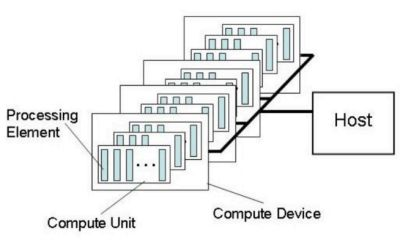
\includegraphics[width=10cm]{fig/opencl_platform_model.jpg}
\caption[OpenCL platform model]{OpenCL platform model with one host and multiple
devices\cite{opencl}.}
\label{oclpm}
\end{figure}


\subsection{Execution Model}
The OpenCL software executes on two levels
\begin{itemize}
\item \textbf{Host code} -- the OpenCL doesn't define any restrictions about the 
host part of the application, it defines only the interaction between host and 
devices. It consists of selection and initialization of the context -- selected 
platform and devices.
\item \textbf{Device code} -- written in OpenCL programming language in the form
of short functions, kernels, that usually transform an input array through 
series of processes into output array. It is compiled via OpenCL compiler and 
executed on the device's work-items.
\end{itemize}

The host program takes care of synchronization and plans the execution of each
kernel on the devices. Each instance of kernel runs in separate work-item and 
the work-items within each work-group execute concurrently. 

\subsection{Memory Model}
OpenCL defines two types of memory objects. The \textit{buffer object} is
versatile type that could be used for representation of any data type 
available in C or OpenCL language. The \textit{image object} is restricted 
to containing pictures only and is optimized for the specific needs of 
image processing.

OpenCL uses a hierarchically structured memory. The types differ in access time,
availability and types of usage\cite{opencl}:
\begin{itemize}
\item \textbf{Private Memory} -- each work-item has it's own private memory 
which could be thought of as analogy to CPU's registers. It is the fastest type 
of memory used in OpenCL.
\item \textbf{Local Memory} -- designed for sharing data between work-items who 
belong to the same work group. It is used to reduce the number of accesses to 
the global memory. Local memory is slower than private memory but faster than 
global memory. The programmer is denied both direct access and control over 
local memory. The analogy could be the cache in CPU.
\item \textbf{Global Memory} -- shared among all work-items in the same context.
\item \textbf{Host Memory} -- memory visible only for the host, OpenCL only 
defines how the host interacts with OpenCL objects and constructs.
\end{itemize}

\hspace{-1.5em}
There could be another type of memory in graphic cards that OpenCL doesn't 
define

\begin{itemize}
\item \textbf{PCI Memory} -- type of memory that could be used by the program 
and GPU, part of host memory. It is slower than global memory.
\end{itemize}



%%%%%%%%%%%%%%%%%%%%%%%%%%%%%%%%%%%%%%%%%%%%%%%%%%%%%%%%%%%%%%%%%%%%%%%%%%%%%%%%
\chapter{Design}\label{chapter:design}%\cite{apu:crypto}
The aim of the implementation is to determine whether the parallel processing
of SRTP could increase the limitations on modern VoIP softgates. The development
of sophisticated softgate requires elaborate engineering and implementation
of various communication protocols that would overshadow the effort in parallel
processing. Therefore only narrow selection of well know communication protocols
has been implemented. For VoIP telephony, registration and maintenance of users
serves \textit{SIP} protocol, for the media transmission description
and session description \textit{SDP} protocol, and for secure media transport 
\textit{SRTP} with \textit{ZRTP}. There is also implementation of \textit{LCP} 
stack\footnote{ Light-weight Control Protocol -- communication protocol for
Siemens prototype VoIP phone.}.


\section{Design Patterns}
More complex the application is the higher level of considerate design it 
requires. There are plenty of already well tested design patterns from
which the implementation could be based on and as the field of VoIP
communication has been known for decent amount of time, there are currently
couple of advised design patterns, from which the particular implementation for 
this thesis stands on four -- mediator pattern, singleton pattern, factory 
method pattern \cite{design-patterns} and protocol stack pattern 
\cite{protocol-stack}. None of these design patterns could be thought as 
contribution of the thesis as they all belong to common public knowledge and 
their examination was not the main topic of the  research. However, their 
explanation is provided in order to make the rest of the chapter more 
comprehensible.

\subsection{Mediator Pattern}
In object oriented design the common problem be the large number of classes and
their mutual interaction. One of the possible solutions for the latter can be
behavioral pattern called mediator, which is named after the way it alters the
running behavior. The pattern consists of following participants:

\begin{itemize}
\item \textbf{Mediator} -- defines an interface for communicating with colleague 
objects
\item \textbf{ConcreteMediator} -- implements cooperative behavior by 
coordinating colleague objects, it knows and maintains its colleagues
\item \textbf{ConcreteColleague} -- each colleague knows its mediator object and
it communicates with its mediator whenever it would have otherwise communicated 
with another colleague
\end{itemize}

The mediator object communicates with multiple colleague object through defined
interface, the interaction between colleague objects is strictly limited.
One of the issues of such design is that the data flow might be bottlenecked by
the only option of mutual communication is realised via single object if there
is a need for critical section and their exclusion.

\subsection{Singleton Pattern}
During creation of the application architecture certain class may be required
to provide global point of access to it while preserving only one instance.
One approach could be to have global variable but that is not complete 
fulfilment of the requests, because multiple instances could still be created. 
Singleton design pattern offers a solution when the class itself is responsible 
for the number of instances which ensures that nowhere in the code multiple 
object of such class may be created. This doesn't affect the rest of the design, 
only one single class, therefore, it has only one participant:

\begin{itemize}
\item \textbf{Singleton} -- there must be exactly one instance of the class and
class must prevent from instantiation of multiple instances,  it must be 
globally available from well known access point
\end{itemize}

%\subsection{Factory Method Pattern}
%\url{http://en.wikipedia.org/wiki/Factory\_method\_pattern}

\subsection{Protocol Stack Pattern}
There are two design patterns closely related to the protocol stack design 
pattern which it uses as higher level of abstraction in explaining the 
correspondign relations in design.
\begin{itemize}
\item \textbf{Protocol Layer} -- provide a common interface for implementing
different layers of communication protocol stack.
\item \textbf{Protocol Packet} -- unification and simplification of internal
packet buffers and their access.
\end{itemize} 

This pattern's usage is concentrated but not limited to dynamic exchange of 
protocol layers from the stack, their insertion and removal, thanks to separate 
view and decoupling of each implemented protocol and its layers.

The participants of protocol stack pattern are:
\begin{itemize}
\item \textbf{Protocol Stack} -- contains and maintains list of used protocols.
\item \textbf{Protocol Layer} -- provides interface and communication point for 
each individual layer. The certain layers are abstracted from the actual type of
the upper layer and lower layer classes.
\end{itemize}


%\url{http://www.eventhelix.com/realtimemantra/PatternCatalog/protocol\_stack.htm#.UYEfRbXQovo}



\section{SIP Gateway}
In order to create a session for VoIP communication between two endpoints, 
there must be device that will be able to create such connection and negotiate
protocols for their interaction and data exchange. In telecommunications such
device is called \textit{gateway}. The essential function of gateway is 
protocol translation to interconnect networks and devices using different
protocol technologies. The SIP gateway used in this thesis provides protocol
conversion between subset of SIP protocol and full implementation of LCP 
protocol.

\begin{figure}[h!]
\centering
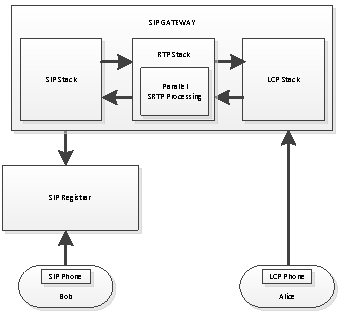
\includegraphics[width=13cm]{fig/scenario1.pdf}
\caption[Gateway scenario]{SIP gateway with two VoIP telephones accessible, LCP 
phone directly connected and SIP phone through SIP Registrar.}
\label{oclpm}
\end{figure}

Multiple SIP or LCP telephones are connected to the SIP Gateway whose appear as
users to the SIP registrar\footnote{ Used registrars were Asterisk and Siemens 
HiPath 4000}. The SIP gateway in this scenario works as bridging point between 
the SIP telephones and SIP registrar, LCP phones and SIP registrar or LCP phones
directly.

The modules of SIP gateway are implemented in different programming languages
and each serve specified purpose.
\begin{itemize}
\item \textbf{Gateway core} -- implemented in Java, provides communication 
between each module and encapsulates basic functionality of a Gateway.
\item \textbf{SIP Stack} -- Java API for SIP stack called 
JAIN SIP\cite{jainsip}, implemented basic SIP features.
\item \textbf{LCP Stack} -- implemented in Java fully covering LCP protocol 
v1.0.
\item \textbf{RTP Stack} -- for non-direct connections where the telephones 
couldn't agree on communication channel for the session, RTP stack implemented
in C/C++ and OpenCL provides necessary bridging point.
\end{itemize}

Measurement of utilization of computational resources during execution of 
ciphering algorithm does provide correct and exact results, however in real 
deployment the effectivity could be negatively affected by the other processes 
running on the softgate. SIP Gateway is a collection of programs and utilities
whose together implement a server for lightweight LCP phones and supplement a
SIP functionality for each phone to be able to connect to an actual SIP 
registrar. 

\begin{figure}[h!]
\centering
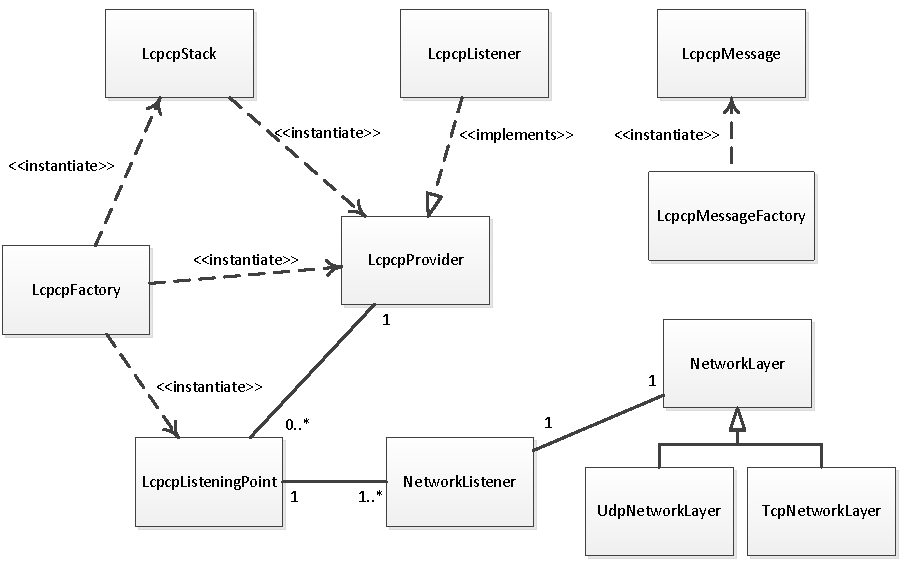
\includegraphics[width=15cm]{fig/lcpstack.pdf}
\caption[LCP stack design]{Architecture of LCP stack, design was inspired by the 
JAIN-SIP api\cite{jainsip}.}
\label{lcpstack}
\end{figure}

\begin{figure}[h!]
\centering
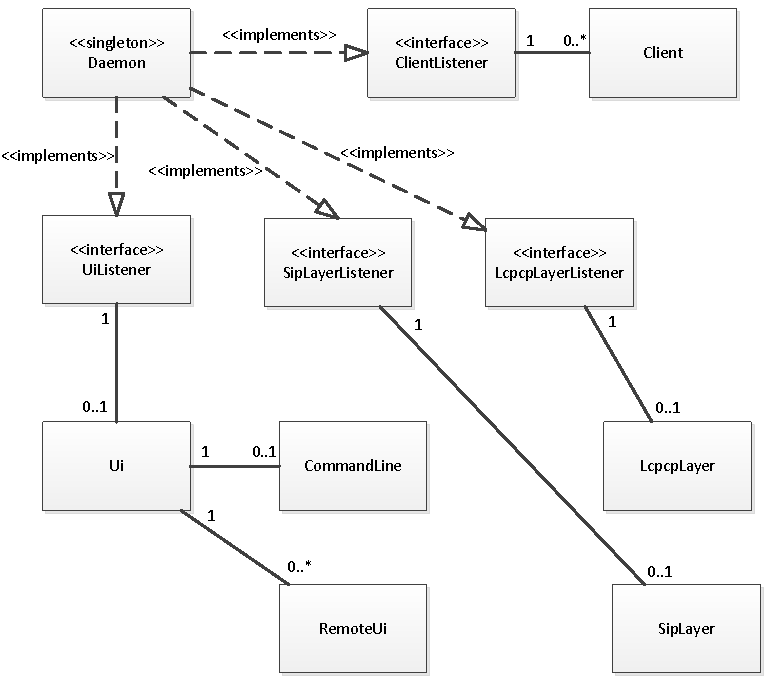
\includegraphics[width=15cm]{fig/sipgw.pdf}
\caption[SIP gateway design]{Architecture of SIP Gateway with singleton design 
pattern. Consists of \textit{Daemon} class, multiple LCP phones connected via 
LCP stack and represented as instances of \textit{Client} class and multiple 
user interfaces for control over the gateway.}
\label{gw}
\end{figure}

The core application should offer simple management via command line for 
both development and tracing of the flowing communication and basic 
functionality for communication and session management. 

The core class of the gateway is \texttt{Daemon}, which controls the flow of 
data inside the application and provides interfaces to communicate with external 
applications. During the composition of gateway the mediator design pattern
was used where the daemon is mediator and all directly communicating classes are
colleagues.
 
\texttt{SIP Stack} provides the interface to communicate with SIP Registrar. 
The single SIP Stack is shared for all users, implicitly runs on well known port
for SIP communication 5060, which could be explicitly changed if necessary.

\texttt{LCP Stack} visualized on the figure \ref{lcpstack} was designed to 
reflect the elaborate design used in JAIN SIP\cite{jainsip}. While SIP is much 
richer protocol than LCP, the design of the stack was extremely shortened but 
the basic structure of elementary components and their interaction remained the 
same. LCP stack runs implicitly on the recommended port 4066, but as well as SIP 
stack port, the port could be variable if needed. Each SIP/LCP client is 
instance of \texttt{Client} class, and universal interface for remote 
communication and administration shall be provided as well.

\texttt{RTP Stack} is devoted increased amount of attention in design because it 
covers the focus of this thesis. All of the stacks are interchangable and during 
their design were used recommendations from protocol stack design pattern and 
its related patterns.


\section{SRTP Stack}
The essential point of implementation improvement lies in design of SRTP stack 
as it has been mentioned in previous text that it consumes majority of resources 
of the gateway during indirect media sessions. Proper implementation must not lack following properties:

\begin{itemize}
\item \textbf{encryption module} -- implementation of AES-128b cipher as defined
in RFC-3711 \cite{rfc3711} in at least CRT mode that provides protection of transferred
data with different keys for each endpoint in all concurrent sessions.
\item \textbf{input and output buffers} -- in order to avoid exhaustive allocation
and deallocation of structures for input and output packets, the data storage should
be implemented as thread safe pool of buffers  with sufficient size and both, 
synchronization techniques and memory override protection.
\item \textbf{transcoding module} -- due to various reasons, endpoints may not be
able of negotiate the same media compressing codec. The SRTP stack should allow
the transcoding and then encapsulate the process without unneccessary additional
demands for the gateway.
\item \textbf{integration interface} -- most of the procedures implemented in
SRTP stack should be encapsulated to minimize overloading data transferres with
the gateway providing only essential and minimal interface with callback
features to simplify and unify the integration process.
\end{itemize}

An advanced techniques like \textbf{jitter buffer} may improve overall quality
of VoIP communication, however, each end device capable of such communication must
implement these techniques as well, therefore, it may render itself redundant 
and generating minimal, but still additional latency.

\subsection{SRTP Processing}
Advantage of usage AES in CM is that it allows out-of-order processing. Because
majority of RTP implementations are build on UDP transport layer, which is 
simple model with minimal protocol mechanisms, neither order nor delivery of the
packets are guaranteed in exchange for smaller average delay and smaller 
traffic. 

The exact size of payload in SRTP packet can differ widely according to the 
used codec, its bit rate, and sampling frequency. The selection of used voice
codecs, their sampling periods and payload size are mentioned in table 
\ref{bandwidth}.

\begin{table}[H]
\begin{center}
\begin{tabular}{|l|ccc|}\hline%
  Codec and Bit Rate & Payload Size & Sampling Period & Packets Per Second\\\hline
  G.711 -- 64 Kbps   & 160 bytes    & 20 ms           & 50 \\
  G.729 -- 8 Kbps    & 20 bytes     & 20 ms           & 50 \\
  G.726 -- 32 Kbps   & 80 bytes     & 20 ms           & 50 \\
  G.726 -- 24 Kbps   & 60 bytes     & 20 ms           & 50 \\
  G.728 -- 16 Kbps   & 60 bytes     & 30 ms           & 33 \\
 \hline
\end{tabular}
\end{center}
\caption[Codec payloads]{Selected codecs and payload information 
\cite{rtpbandwidth}.}
\label{bandwidth}
\end{table}

Fixed block size of AES is 16 bytes, which means that one or more states could
be mapped to the packet using any of the mentioned common codecs. Parallelization
of the encryption process could be performed either on a single state, where
value during every method of the AES of each cell of the state is computed 
separately, therefore a work-item can be mapped on computing for each cell. 
Theoretical common hardware should be capable of utilizing 16 work-items in a 
single work-group which is the maximal number of needed by this design.

Another possible approach for codecs with larger payload size, such as G.711, 
could be to map multiple states for the parallel execution of entire packet, 
which for the particular codec would require significantly more computational 
units. 

\vspace{1em}

\begin{figure}[h!]
\centering
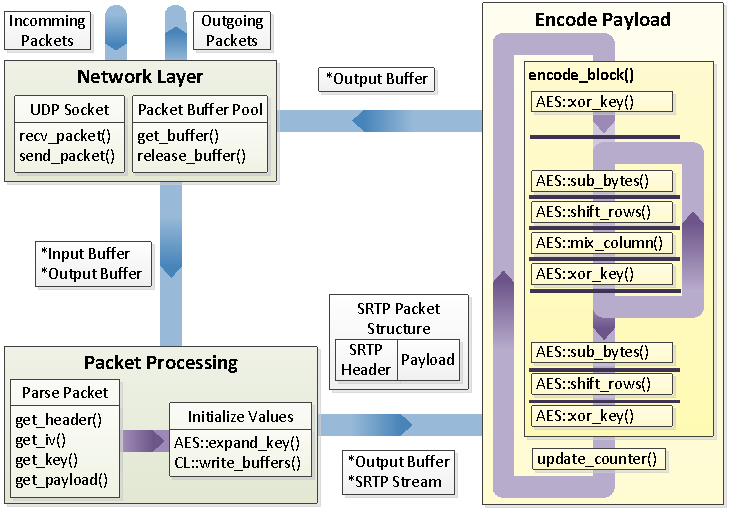
\includegraphics[width=15cm]{fig/paral_scheme.pdf}
\caption[SRTP processing scheme]{SRTP processing scheme.}
\label{scheme}
\end{figure}

The SRTP processing scheme from figure \ref{scheme} visualizes the ideas behind
the design of SRTP stack and encapsulates implementation details for easier
explanation from the multi-threaded application design point of view. 
The entire stack runs in three separate threads which shall minimize the delay 
caused by waiting on modules with varying time of execution per packet.
\begin{itemize}
\item \textbf{Network Thread} -- the incoming and outgoing data are captured
via two sockets, for RTP and RTCP. This thread includes a pool of buffers for
the storage of packets and another the processed data.
\item \textbf{Stack Thread} -- the interaction and selection attributes for
the processing thread is taken care in the stack thread as well as interface
for higher layers of the application using the SRTP stack.
\item \textbf{Packet Processing Thread} -- extraction of important values from
the packet header, encoding and decoding provided with transcoding interface of 
the entire packet payload according to the previously extracted data.
\end{itemize} 

The thread design could be mapped to another type of view on the layers of
the stack design. The SRTP layers as shown in the scheme \ref{scheme} are subset
of the entire SRTP stack functionality and the classes from the scheme have 
following purposes:

\begin{itemize}
\item \textbf{Network Layer} -- enables the communication with external devices
through SRTP protocol, transfere of the multimedia data packets between endpoints
and implements buffer pool for packet data.  
\item \textbf{Packet Processing Layer} -- without unneccessary data reallocation
the proper structures are casted for easier readability and extraction of important
data from the incomming packets. 
\item \textbf{Payload Encoding} -- complete implementations of encryption and 
decryption of the packet payload.
\end{itemize}

\subsubsection*{Serial Processing}
The designed application captures data from network in the network layer which
ensures communication with both endpoints of multimedia session and is running 
in its own thread. It contains buffer pools for incoming and outgoing data to 
ensure maximal level of parallelization in each layer of application. Pointers 
for input and output buffers are passed for further packet processing where are 
extracted information such as header and payload from the packet, copied data 
from the memory to OpenCL data structures and serial implementation of AES key 
schedule. 

For better understanding of improvement this thesis is provided with reference
serial implementation which design will be analyzed as well. The payload 
encryption design as visualized in figure \ref{scheme} shows, that the execution
is separated into multiple consecutive callings of AES algorithm with updating
of counter in between for CTR mode. Thanks to the decomposition of the code,
the design of parallel encryption is done in similar fashion.

The design prevents the executing implementations from creating any additional
temporary buffers to decrease unnecessary allocations. These can be predicted in
the startup of SRTP stack and already preallocated with maximal size a packet
can have. This approach consumes more memory, but improves memory management and
saves execution time during critical sections. Also it is assumed that softgate
gateway code runs on machine with enough memory and these buffers most certainly
shouldn't mean any excessive memory consumption. 

The buffer pools provided are used in both serial and parallel encryption,
and to increase the level of algorithm categorization, their implementation is
based on template classes. The pool guarantees to protect buffer from overwrite
and data persistency.


\newpage

\subsubsection*{Massive Parallel Processing}
Traditional parallel programming style relies heavily on SIMT\footnote{ SIMT -- 
Single Instruction Multiple Thread} and SPMD\footnote{ SPMD -- Single Program
Multiple Data} programming paradigms \cite{Flynn:1972}. The native OpenCL 
approach is based on abstracting the units of work from the programmers code 
into virtual threads -- work-items. The convenience it offers in allocation
of resources brings couple of limitations as well. 

The figure \ref{mp_payload} demonstrates the processing of packet payload of 
G.711 codec on the chip with work-group size 16. Workload on the work-items can
be highly irregular and each work-item execution is finished after the 
processing of the particular AES block, therefore, this code will need 160
invocations of work-items during the kernel execution. That would bring
unnecessary computational overhead.    

\begin{figure}[H]
\centering
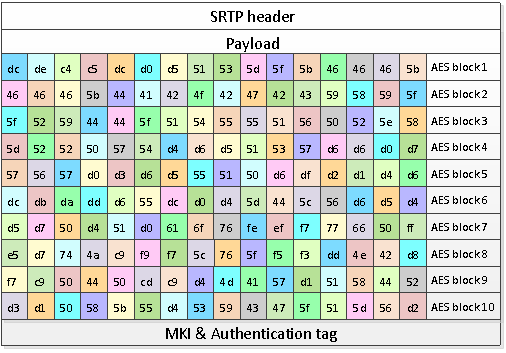
\includegraphics[width=12cm]{fig/packet_mp.pdf}
\caption[OpenCL work-item mapping]{Work-item mapping on packet payload with 
native OpenCL approach.}
\label{mp_payload}
\end{figure}



\subsubsection*{Persistent Thread Processing}
The requirements and attributes imposed by massive parallel processing
style divide the workload into multiple blocks, more than can be simultaneously
executed during kernel launch time, and the synchronization is ensured by the
OpenCL. For massive parallel applications the obvious approach would be to 
utilize as much of machine's power as possible to gain the largest speed-up in 
every single execution. However, the aim of this thesis is to minimize large 
delays for multiple sessions which requires rather careful allocation of
resources. Persistent threads is special type of programing paradigm combining 
both, the possible gain of mapping the program for parallel computation and
considerate usage of resources \cite{pt}.

Since the initialization of computational kernel can consume significant amount 
of time compared to the actual execution, larger kernel reusing its resources 
for multiple similar computations could render the initialization negligible 
trading off portion of parallelization. This approach has been chosen for
packet parsing, while instead of mapping 160 OpenCL work-items on the G.711 
packet's payload it uses one work-item for each AES block cell in a loop that 
goes through the data.

Maximal simultaneous work-items launched during the kernel execution is equal
to the number of blocks in AES algorithm and it must not be larger than the
amount of work-items in work-group. The persistent thread style provides 
couple of relevant improvements that are not resolved in common parallel 
implementation to the satisfactory degree.

\begin{itemize}
\item \textbf{Global synchronization} -- as the kernel uses only as many 
work-items as can be simultaneously scheduled, the tools OpenCL offers
for synchronization within work-group can be used to synchronize calculations
through the entire execution at any given point which is used in 
synchronization across AES blocks for update of \textit{round key}.
\item \textbf{Computational overhead} -- the amount of computations in a 
work-item for 128-bit AES is larger than initialization, startup and cleanup
of the kernel, but those factors are not completely insignificant. Limiting
the number of consecutive executions decreases the ratio of OpenCL overhead and
the algorithm performance in positive way.
\item \textbf{Resource requirement consistency} -- memory requirements are
similar for both persistent thread and massive parallel style, but size of the 
payload for single packet may consume up to 160 work-items on the GPU if kernel
is programmed in non persistent thread style. As it doesn't seem to be much for
one packet, if the stack should take care of multiple SRTP streams, the 
resources may promptly become insufficient which will increase the weight of 
OpenCL overhead. Persistent thread kernel will not use more than 16 work-items
per packet.
\end{itemize}

\begin{figure}[H]
\centering
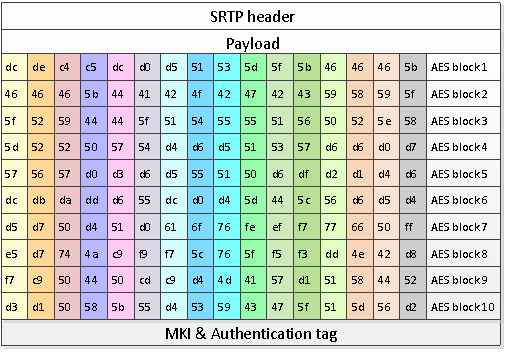
\includegraphics[width=12cm]{fig/packet_wi.pdf}
\caption[Persistent thread work-item mapping]{Work-item mapping on packet 
payload using persistent thread paradigm.}
\label{pt_payload}
\end{figure}


\section{Transcoding}
Essential part of the media server is ability to negotiate the best codec for
both endpoints in real-time media session. When all participating devices can
not communicate using the same compressing media codec, the gateway must be able
of transcoding to provide the channel for communication. RTP protocol defines
127 different codecs for audio and video profile. Therefore, the designed 
SRTP stack uses plugin system for multimedia codec transcoding.

The design of plugin system takes into consideration the lifetime of packet data 
buffers and  for optimization purposes may defer the release of buffers on the 
side of codec plugin. The core desing is simple and consists of two parts.

\begin{itemize}
\item \textbf{Plugin System Module} -- part of the gateway, on the startup 
browses defined directory for any plugins and dynamically links them into the 
application. The plugin system may offer the management of packet memory buffers
on the side of codec plugin, but the system doesn't guarantee the consistency 
through the entire lifetime and if necessary, the buffer may be rewritten, in 
which case the flag for data correctness is set off. 
\item \textbf{Codec Plugin} -- compiled files implementing the plugin interface
capable at least of both transcoding the codec from and into PCM \footnote{ PCM 
-- Pulse-code modulation.} and preferably also optimized transcoding into
another codec, if such algorithm is presented. The codec plugin is responsible
for implementing or control of any buffers if necessary, concurrently transcode 
multiple different streams, and must separate the buffers and another saved 
information from given stream ID. The plugin may not use the optimization 
option, duplicate the data into its own buffers and keep the memory management
on the part of SRTP stack itself.  
\end{itemize}  

\begin{figure}[H]
\centering
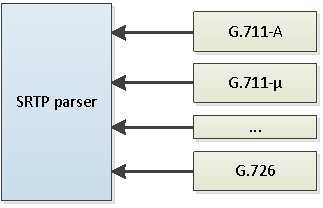
\includegraphics[width=9cm]{fig/plugins.pdf}
\caption[Plugin system design]{Interaction between plugin system on the gateway 
and separate codec plugins.}
\label{pt_payload}
\end{figure} 


%%%%%%%%%%%%%%%%%%%%%%%%%%%%%%%%%%%%%%%%%%%%%%%%%%%%%%%%%%%%%%%%%%%%%%%%%%%%%%%%
\chapter{Implementation}\label{chapter:implementation}
The application's specifications were variable through the life-cycle of the 
entire development. SIP gateway's implementation started as a prototype for 
translating LCP protocol and subset of SIP protocol enabling basic functionality 
for  new lighweight prototype telephones. As the statement of requirements 
included reference Java application that combined LCP server and multiple SIP 
clients,  the implementation languages differ from the SRTP stack which is the 
core of this thesis.

As mentioned before, the reference application implements only a subset of 
the full communication protocols and instead of understanding all of the complex
scenarios the protocols offer, it brings research value examining 
the  possibilities of improvement implementing computationally demanding 
algorithms using parallel programming paradigm. Another benefit this work 
brings, is experimental study and comparison of established implementations used
either commercially or free.

\lstset{ %
language=C++,                        % choose the language of the code
basicstyle=\footnotesize\tt,   % the size of the fonts that are used for the code
numbers=left,                   % where to put the line-numbers
numberstyle=\footnotesize,      % the size of the fonts that are used for the line-numbers
stepnumber=1,                   % the step between two line-numbers. If it is 1 each line will be numbered
numbersep=10pt,                  % how far the line-numbers are from the code
backgroundcolor=\color{light-gray},  % choose the background color. You must add \usepackage{color}
showspaces=false,               % show spaces adding particular underscores
showstringspaces=false,         % underline spaces within strings
showtabs=false,                 % show tabs within strings adding particular underscores
%frame=single,           % adds a frame around the code
tabsize=2,          % sets default tabsize to 2 spaces
captionpos=b,           % sets the caption-position to bottom
breaklines=true,        % sets automatic line breaking
breakatwhitespace=false,    % sets if automatic breaks should only happen at whitespace
escapeinside={\%*}{*)},          % if you want to add a comment within your code
keywordstyle=\bf\color{blue},
commentstyle=\color{gray},
stringstyle=\color{red},
escapechar=@,
morekeywords={BYTE, CBYTE, nullptr, __local},
}

%\begin{figure}[H]
%\begin{lstlisting}
%@\color{brown}{\#define CONST 16}@                         //komentar
%void funkce(int param, int param2){   //komentar2
%  int a = @\color{red}{0x05}@;
%  int b = @\color{brown}{CONST};
%}
%\end{lstlisting}
%\end{figure}

\section{SIP Gateway}
\subsection{SIP Layer}
\subsection{LCP Layer}


\section{SRTP Stack}
Lorem ipsum dolor sit amet, consectetuer adipiscing elit. Pellentesque pretium lectus id turpis. Fusce wisi. Nunc tincidunt ante vitae massa. Nulla non lectus sed nisl molestie malesuada. Nulla quis diam. Cras pede libero, dapibus nec, pretium sit amet, tempor quis. Phasellus enim erat, vestibulum vel, aliquam a, posuere eu, velit. Curabitur ligula sapien, pulvinar a vestibulum quis, facilisis vel sapien. Quisque tincidunt scelerisque libero.


\subsection{Buffer Pool}
Lorem ipsum dolor sit amet, consectetuer adipiscing elit. Pellentesque pretium lectus id turpis. Fusce wisi. Nunc tincidunt ante vitae massa. Nulla non lectus sed nisl molestie malesuada. Nulla quis diam. Cras pede libero, dapibus nec, pretium sit amet, tempor quis. Phasellus enim erat, vestibulum vel, aliquam a, posuere eu, velit. Curabitur ligula sapien, pulvinar a vestibulum quis, facilisis vel sapien. Quisque tincidunt scelerisque libero.

\begin{figure}[H]
\begin{lstlisting}
template <class buffer_item> class Buffer_pool {
    private: //implementation
        buffer_item **pool = nullptr;
        std::queue<int> free_buffer_index;
        int pool_size;

    public: //interface
        // initialize pool and free_buffer_index
        Buffer_pool(int pool_size) { .. };
        // cleanup of resources
        ~Buffer_pool() { .. };
        // returns available buffer ID
        int get_buffer_id() { .. };
        // returns size of pool
        int get_pool_size(){ .. };
        // returns available buffer with ID
        buffer_item* get_item(int id) { .. };
        // makes buffer with ID available
        void release_buffer(int id) { .. };
};
\end{lstlisting}
\end{figure}

To achieve higher degree of code reusability and categorization, buffer pool
is implemented as template class offering both the OpenCL implementation
use its own pool for memory objects on the host side and network interface
use its own pool for incomming and outgoing packets and their structures.

\begin{figure}[H]
\begin{lstlisting}
class RTP_item {
    public:
        RTP_item();
        ~RTP_item();
        // packet data buffers
        BYTE src[@\color{brown}{PACKET\_SIZE@];
        BYTE *payload_src;
        BYTE dst[@\color{brown}{PACKET\_SIZE}@];
        BYTE *payload_dst;
        BYTE temp[@\color{brown}{PACKET\_SIZE}@];
        // IPv6 BSD socket structures
        struct sockaddr_in6 src_addr;
        struct iovec iov[@\color{red}{1}@];
        struct msghdr msg;
};
\end{lstlisting}
\end{figure}

The buffer pool item for network packets includes the buffers for incomming and 
outgoing packets and the pointers to payload to avoid perpetual header removal.
Network interface uses GNU C standard implementation of BSD sockets, therefore,
this item includes structures for the sockets as well to keep the information
persistent through packet processing.

\begin{figure}[H]
\begin{lstlisting}
class cl_item{
    public:
        cl_mem payload_src; //buffer for payload
        cl_mem payload_dst;
        cl_mem iv_gpu;      //buffer for initial vector
        cl_mem rk;          //round key
        cl_mem t1;          //auxiliary buffers
        cl_mem t2;
};
\end{lstlisting}
\end{figure}

OpenCL requires specific memory objects that can be loaded to the device memory.
Buffer pool item for parallel implementation requires only those memory objects.


\subsection{AES}
For the SRTP stack the crucial is implementation of Advanced Encryption Standard.
Described are two most relevant implementations, serial for comparison with
the current solutions and persistent thread as the representative of the the
best examined parallel implementation.

The header file \texttt{aes.h} offers the functions for encryption and 
decryption of packet payload in CTR mode encapsulated in \texttt{AES} namespace.

\subsubsection*{Key Schedule}
The master key defined for every SRTP session must be expanded into round key,
which is used in every round for encryption. The algorithm for round key schedule
is provided only in serial implementation, because its execution is prompt and
doesn't provide enough calculations for the kernel device that would justify
parallel implementation and diminish OpenCL computational overhead.

\begin{figure}[H]
\begin{lstlisting}
//precomputed rcon table
static const BYTE rcon[]     = {@\color{red}{0x8d}@, ... };
//key expansion
void AES::expand_key(BYTE *mk, BYTE rk[@\color{brown}{ROUND\_KEY\_SIZE}@][@\color{brown}{BLOCK\_SIZE}@]){
    get_first_rk(mk, rk[@\color{red}{0}@]);
    for(int i = @\color{red}{1}@; i<@\color{brown}{ROUND\_KEY\_SIZE}@; i++){
        get_next_rk(mk[i-@\color{red}{1}@], rk[i], rcon[i]);
    }
}
\end{lstlisting}
\end{figure}

Key expansion algorithm is different for the first round key and the rest of
round keys. Both methods are described in this chapter.
 
\begin{figure}[H]
\begin{lstlisting}
void get_first_rk(BYTE *key, BYTE *rk){
    memcpy(rk, key, @\color{red}{16}@*sizeof(BYTE));
}
\end{lstlisting}
\end{figure}

The first round key is copy of first 128 bits from the master key. 

\begin{figure}[H]
\begin{lstlisting}
void get_next_rk(BYTE *previous_key, BYTE *rk, BYTE rcon){
    rotate_column(previous_key, rk, @\color{red}{0}@, @\color{red}{3}@, @\color{red}{1}@);
    for(int r = 0; r<@\color{brown}{ROWS}@; r++){
       rk[r*@\color{brown}{COLUMNS}@] = sbox[rk[r*@\color{brown}{COLUMNS}@]] ^ previous_key[r*@\color{brown}{COLUMNS}@]; 
    }
    rk[@\color{red}{0}@] = rk[@\color{red}{0}@] ^ rcon;
    for(int c = @\color{red}{1}@; c<@\color{brown}{COLUMNS}@; c++){
        for(int r = @\color{red}{0}@; r<@\color{brown}{ROWS}@; r++){
            rk[r*@\color{brown}{COLUMNS}@+c] = previous_key[r*@\color{brown}{COLUMNS}@+c] ^ rk[r*@\color{brown}{COLUMNS}@+c-@\color{red}{1}@];
        }
    }
}
\end{lstlisting}
\end{figure}
Other round keys are derived from the previous round key. The algorithm is 
devided into two steps, first calculates the first column of the key state
and then are calculated columns two, three and four always derived from
the previous column. Because every array in the SRTP stack is considered
one dimensional exactly as the incomming packet, the index to the state matrix
memory must be computed exclusively.

\subsubsection*{Serial Encryption}
The AES encryption is divided into 4 steps exactly as described in previous
chapters. Five constants necessary for AES will be mentioned through this 
chapter in many code snippets and are listed in the following algorithm for 
encryption. Their definitions are later skipped to avoid information redundancy.

\begin{figure}[H]
\begin{lstlisting}
//AES constants
@\color{brown}{\#define ROUND\_KEY\_SIZE 11}@ 
@\color{brown}{\#define ROUNDS \hspace{30pt} 10}@ 
@\color{brown}{\#define BLOCK\_SIZE \hspace{13pt} 16}@ 
@\color{brown}{\#define ROWS \hspace{44pt} 4}@ 
@\color{brown}{\#define COLUMNS \hspace{30pt} 4}@ 
//CTR encryption algorithm
void AES::srtp_encode(BYTE *src, BYTE *dst, BYTE *key, BYTE *iv, int len){
    xor_key(key,iv,key);
    expand_key(key,round_key);
    int i = @\color{red}{0}@, j = @\color{red}{0}@;
    int last_offset = len/@\color{brown}{BLOCK\_SIZE}@*@\color{brown}{BLOCK\_SIZE}@;
    //encryption of counter and XORing with blocks
    for( ; i < length; i+=@\color{brown}{BLOCK\_SIZE}@){
        encode_block(counter, dst+i, round_key);
        xor_key(dst+i,dst+i,src+i);
        update_counter(counter);
    }
    //encryption of counter is full but XORing only up to packet size
    BYTE *last_block = dst+last_offset;
    encode_block(counter, last_block, round_key);
    for(i=i-@\color{brown}{BLOCK\_SIZE}@; i < length; i++, j++){
        dst[i] = last_block[j] ^ src[i];
    }
}
\end{lstlisting}
\end{figure}

The function takes five arguments, four of those are input parameters and one
is output, result of the encryption. The first argument \texttt{src} is pointer
to the buffer with packet payload that needs to be encrypted, \texttt{dst} is
pointer to the buffer with outgoing packet payload after encryption, arguments
\texttt{key} and \texttt{iv} represent encryption properties and finally the
last argument \texttt{len} has length of the packet payload.

\begin{figure}[H]
\begin{lstlisting}
void encode_block(BYTE *counter, BYTE *dst, BYTE **round_key){
    BYTE temp[@\color{brown}{BLOCK\_SIZE}@];
    xor_key(counter, temp, round_key[@\color{red}{0}@]);
    for(int i = @\color{red}{1}@; i < @\color{brown}{ROUNDS}@; i++){
        sub_bytes(temp, dst);
        shift_rows(dst, temp);
        mix_columns(temp, dst);
        xor_key(dst, temp, round_key[i]);
    }
    sub_bytes(temp,dst);
    shift_rows(dst,temp);
    xor_key(temp,dst,round_key[@\color{brown}{ROUNDS}@]);
}
\end{lstlisting}
\end{figure}

Implementation of the block encode follows the algorithm described in chapter
\ref{chapter:srtp} in algorithm \ref{encr}. Since the CTR mode encrypts the
counter, packet payload doesn't have to be present. 

\begin{figure}[H]
\begin{lstlisting}
//precomputed AES tables
static const BYTE g2[] = {@\color{red}{0x00}@, ... };
static const BYTE g3[] = {@\color{red}{0x00}@, ... };
//optimized multiplication in Galois field
void mix_columns(BYTE *src, BYTE *dst){
    BYTE a0, a1, a2, a3;
    for(int col = @\color{red}{0}@; col < @\color{brown}{COLUMNS}@; col++){ 
        a0 = src[col]; 
        a1 = src[col+@\color{red}{4}@];
        a2 = src[col+@\color{red}{8}@];
        a3 = src[col+@\color{red}{12}@];
        //using precomputed tables
        dst[col]    = g2[a0] ^ g3[a1] ^ a2     ^ a3;
        dst[col+@\color{red}{4}@] @\hspace{0.9pt}@ = a0     ^ g2[a1] ^ g3[a2] ^ a3;
        dst[col+@\color{red}{8}@] @\hspace{0.9pt}@ = a0     ^ a1     ^ g2[a2] ^ g3[a3];
        dst[col+@\color{red}{12}@]@\hspace{1.9pt}@ = g3[a0] ^ a1     ^ a2     ^ g2[a3];
    }
}
\end{lstlisting}
\end{figure}
The multiplication in Galois field by matrix defined in chapter 
\ref{chapter:srtp} is computationally expensive, therefore, the implementation
consits of precomputed values stored in arrays and then the mixture of columns.

\begin{figure}[H]
\begin{lstlisting}
void xor_key(BYTE *src, BYTE *dst, BYTE *key){
    for(int i = @\color{red}{0}@; i < @\color{brown}{BLOCK\_SIZE}@; i++){
        dst[i] = src[i] ^ key[i];
    }
}
\end{lstlisting}
\end{figure}



\begin{figure}[H]
\begin{lstlisting}
void shift_rows(BYTE *src, BYTE *dst){   
    for(int row = @\color{red}{0}@; row < @\color{brown}{ROWS}@; row++){
        rotate_row(src+(row*@\color{brown}{COLUMNS}@), dst+(row*@\color{brown}{COLUMNS}@), row);
    }
}
\end{lstlisting}
\end{figure}

Both \texttt{xor\_key()} and \texttt{shift\_rows()} are simple and selfexplanatory
functions. The \texttt{shift\_rows} uses helper function \texttt{rotate\_row()}.

\begin{figure}[H]
\begin{lstlisting}
static const BYTE sbox[] = {@\color{red}{0x63}@, ... };
void sub_bytes(BYTE *src, BYTE *dst){
    for(int i = @\color{red}{0}@; i < @\color{brown}{BLOCK\_SIZE}@; i++){
        dst[i] = sbox[src[i]];
    }
}
\end{lstlisting}
\end{figure}


Following are two helper functions for AES algorithm that are neither described 
in the theoretical part of the thesis nor the AES definition document. Their
implementation has single purpose -- higher code readability.

\begin{figure}[H]
\begin{lstlisting}
void rotate_row(BYTE *src, BYTE *dst, int n){
    int max = @\color{brown}{COLUMNS}@-n;
    for(int i = @\color{red}{0}@; i < max; i++){
        dst[i] = src[i+n];    
    }
    for(int i = max; i < @\color{brown}{COLUMNS}@; i++){
        dst[i] = src[i-max];
    }
}
\end{lstlisting}
\end{figure}

The values in a row specified by arguments \texttt{src} and \texttt{dst} as 
pointers to the particular row in both blocks are rotated by the value 
\texttt{n}. Code is split into two cycles when both together cycle through the 
particular row only once. 

\begin{figure}[H]
\begin{lstlisting}
void rotate_column(BYTE *src, BYTE *dst, int col1, int col2, int n){
    int max = @\color{brown}{ROWS}@-n;
    for(int i = @\color{red}{0}@; i < max; i++){
        dst_state[i*@\color{brown}{COLUMNS}@ + col1] = src_state[(i+n)*@\color{brown}{COLUMNS}@ + col2];
    }
    for(int i = max; i < @\color{brown}{ROWS}@; i++){
        dst_state[i*@\color{brown}{COLUMNS}@ + col1] = src_state[(i-max)*@\color{brown}{COLUMNS}@ + col2];
    }
}
\end{lstlisting}
\end{figure}

Because AES block is stored in the linear memory by rows, when rotating columns
it won't be sufficient to pass the pointer to specific column. Therefore,
the function takes arguments \texttt{col1} as index of column in \texttt{src}
block and \texttt{col2} as index of column in \texttt{dst} block. The argument
\texttt{n} again defines the distance for rotation.
 
\subsubsection*{Parallel Encryption}
Code for parallel encryption consists mostly of the kernel code in OpenCL 
language executed in device. The code for host is large but programmed rutines are
common and doesn't display any efforts of improvement and own contribution.

Again the AES tables are precomputed and stored in constant memory space which 
is cached. As a result, a read from constant memory shouldn't cost more than one
read from device memory on a cache miss. For the persisten thread reading from 
the constant cache is as fast as reading from a register as long as all threads 
read the same address.


\begin{figure}[H]
\begin{lstlisting}
//AES block encryption
void encode_block(BYTE *counter, BYTE *dst, BYTE **round_key){
    BYTE temp[@\color{brown}{BLOCK\_SIZE}@];
    xor_key(counter, temp, round_key[@\color{red}{0}@]);
    for(int i = @\color{red}{1}@; i < @\color{brown}{ROUNDS}@; i++){
        sub_bytes(temp, dst);
        shift_rows(dst, temp);
        mix_columns(temp, dst);
        xor_key(dst, temp, round_key[i]);
    }
    sub_bytes(temp,dst);
    shift_rows(dst,temp);
    xor_key(temp,dst,round_key[@\color{brown}{ROUNDS}@]);
}
\end{lstlisting}
\end{figure}

The round key schedule was moved from the kernel to host code. Other lines are
similar to the serial code.

\begin{figure}[H]
\begin{lstlisting}
void encode_block(__local BYTE *counter, __local BYTE *dst, 
                  __local BYTE *temp, __local BYTE *round_key){
    xor_key(counter, temp, round_key);
    barrier(@\color{brown}{CLK\_LOCAL\_MEM\_FENCE}@); 
    for(int i = @\color{red}{1}@; i < @\color{brown}{ROUNDS}@; i++){
        sub_bytes(temp, dst);
        barrier(@\color{brown}{CLK\_LOCAL\_MEM\_FENCE}@);
        shift_rows(dst, temp);
        barrier(@\color{brown}{CLK\_LOCAL\_MEM\_FENCE}@);
        mix_columns(temp, dst);
        barrier(@\color{brown}{CLK\_LOCAL\_MEM\_FENCE}@);
        xor_key(dst, temp, round_key+(i*@\color{brown}{BLOCK\_SIZE}@));
        barrier(@\color{brown}{CLK\_LOCAL\_MEM\_FENCE}@);
    }
    sub_bytes(temp,dst);
    barrier(@\color{brown}{CLK\_LOCAL\_MEM\_FENCE}@);
    shift_rows(dst,temp);
    barrier(@\color{brown}{CLK\_LOCAL\_MEM\_FENCE}@);
    xor_key(temp,dst,round_key+(@\color{brown}{ROUNDS}@*@\color{brown}{BLOCK\_SIZE}@));
}
\end{lstlisting}
\end{figure}

Encoding the block requires local synchronization which is achieved by
\texttt{barrier()} function. Each step of the algorithm may start computations
after the previous step has been finished for all work-items.

\begin{figure}[H]
\begin{lstlisting}
void xor_key(__local BYTE *src, __local BYTE *dst, __local BYTE *key){
    int i = get_global_id(@\color{red}{0}@);
    dst[i] = src[i] ^ key[i];
}
\end{lstlisting}
\end{figure}

Because both global and local ID of the work-item is cached, calling function 
\texttt{get\_global\_id()} doesn't bring any slack-off, therefore, it is not 
necessary to pass the work-item ID to the functions of AES implementation.

\begin{figure}[H]
\begin{lstlisting}
void mix_columns(__local BYTE *src, __local BYTE *dst){
    int i = get_global_id(@\color{red}{0}@);
    int row = i/@\color{red}{4}@;
    int col = i%@\color{red}{4}@;
    BYTE a0 = src[col]; 
    BYTE a1 = src[col+@\color{red}{4}@];
    BYTE a2 = src[col+@\color{red}{8}@];
    BYTE a3 = src[col+@\color{red}{12}@];
    // mix only the byte this work-item belongs to
    if(row == @\color{red}{0}@){
        dst[i] = g2[a0] ^ g3[a1] ^ a2     ^ a3;
    } else if(row == @\color{red}{1}@) {
        dst[i] = a0     ^ g2[a1] ^ g3[a2] ^ a3;
    } else if(row == @\color{red}{2}@) {
        dst[i] = a0     ^ a1     ^ g2[a2] ^ g3[a3];
    } else if(row == @\color{red}{3}@) {
        dst[i] = g3[a0] ^ a1     ^ a2     ^ g2[a3];
    }
}
\end{lstlisting}
\end{figure}

The work-item during kernel execution must identify itself and then find out to 
which branch of code it belongs.

\begin{figure}[H]
\begin{lstlisting}
void sub_bytes(__local BYTE *src, __local BYTE *dst){
    int i = get_global_id(@\color{red}{0}@);
    dst[i] = sbox[src[i]];
}
\end{lstlisting}
\end{figure}

\begin{figure}[H]
\begin{lstlisting}
void shift_rows(__local BYTE *src, __local BYTE *dst){   
    int i = get_global_id(@\color{red}{0}@);
    int row = i/@\color{red}{4}@;
    int col = i%@\color{red}{4}@;
    // shift only the byte this work-item belongs to
    if(row == @\color{red}{0}@){
        dst[i] = src[i];
    } else if(row == @\color{red}{1}@) {
        if(col == @\color{red}{3}@)
            dst[i] = src[i-@\color{red}{3}@];
        else
            dst[i] = src[i+@\color{red}{1}@];
    } else if(row == @\color{red}{2}@) {
        if(col <= @\color{red}{1}@)
            dst[i] = src[i+@\color{red}{2}@];
        else
            dst[i] = src[i-@\color{red}{2}@];
    } else if(row == @\color{red}{3}@) {
        dst[i] = src[i-@\color{red}{1}@];
    }
}
\end{lstlisting}
\end{figure}

The kernel code requires work-item categorization again as the rows shifting 
doesn't provide any means for generalization. This branching in mentioned device
code doesn't bring any additional computations nor increase overhead.

\subsection{Transcoding}
The plugin system was implemented with usage of the GNU C Library. All of the 
important functions for run-time dynamic loading are included from header
\texttt{dlfcn.h}.

\begin{itemize}
\item \texttt{dlopen()} -- loads dynamic library file with \texttt{RTLD\_GLOBAL}
and \texttt{RTLD\_NOW} flags set to make the symbols available for subsequently 
loaded libraries and perform eager symbol resolution. 
\item \texttt{dlsym()} -- returns address where the particular symbol is loaded
into memory.
\item \texttt{dlclose()} -- unloads the dynamic library.
\end{itemize}

The plugin module searches folder \texttt{plugins} for any file ending with 
extension \texttt{.so} and performs plugin test whether the file contains
necessary properties.

\begin{figure}[H]
\begin{lstlisting}
@\color{brown}{PAYLOAD\_TYPES 127}@ //[RFC3551]
// structure for codec plugin
struct Codec {
    int PT = @\color{red}{-1}@;
    char* encoding_name = nullptr;
    int (*transcode)(BYTE *src, BYTE *dst, int l1, int *l2, int pt, int id);
    void (*to_raw)(BYTE *src, BYTE *raw, int l1, int *l2, int id);
    void (*from_raw)(BYTE *raw, BYTE *dst, int l1, int *l2, int id);
};
// list of plugins
static Codec transcode_plugins[PAYLOAD_TYPES];
// transcode module interface
int transcode(BYTE *src, BYTE *dst, //packet buffers 
              int l1, int *l2,      //data lengths
              int pt1, int pt2,     //codec types
              int id);              //stream ID
\end{lstlisting}
\end{figure}

The code sniplet above defines the structure for loaded codec plugins on the 
host application side and interface for plugin module and rest of the SRTP 
stack. Transcoding is always executed through \texttt{transcode()} function and
never directly, because the function handles the possibilities of plugins
and selects the option with best effort ratio and in the worst case transcodes
through PCM.

\begin{figure}[H]
\begin{lstlisting}
// codec identification [RFC3551]
extern const char* encoding_name;
extern const int PT;
// transcodes multimedia data from one codec to another codec
int transcode(BYTE *src, BYTE *dst, int l_src, int *l_dst, int pt, int id);
// transcodes codec to raw PCM
void to_raw(BYTE *src, BYTE *raw, int len_src, int *len_dst, int id);
// transcodes raw PCM to codec
void from_raw(BYTE *raw, BYTE *dst, int len_src, int *len_dst, int id);
\end{lstlisting}
\end{figure}

The plugin must define all of the mentioned interface values and functions.
To ensure proper implementation, each codec plugin includes header file 
\texttt{transcode\_plugin.h}.


\section{Visualization Tool}






%%%%%%%%%%%%%%%%%%%%%%%%%%%%%%%%%%%%%%%%%%%%%%%%%%%%%%%%%%%%%%%%%%%%%%%%%%%%%%%%
\chapter{Results}\label{chapter:results}
One of the major delays caused on gateway during indirect calls is due to
encryption and transcoding. Since the core of this thesis was parallelization
of SRTP encryption, the tests and measurements focus on gathering relevant
information regarding especially the correct usage of SRTP on the gateway. Even
though AES was designed to be fast algorithm, while executed on large amount of
flowing data it can cause measurable overhead.

For the purposes of this chapter there was designed loadtest with following
attributes:
\begin{itemize}
\item each test fulfilled these properties:
\vspace{-0.5em}
\begin{itemize}
\item 300 subscribers executing the calls
\item 50 to 150 concurrent calls in the same time\cite{hp4k}
\item BHCA 2000\footnote{ BHCA -- busy hour call attempts}
\end{itemize}
\item each call from the tests mentioned above:
\vspace{-0.5em}
\begin{itemize}
\item lasted 20 seconds
\item used G.711-a or G.711-$\mu$ codec
\item needed encryption of SRTP
\end{itemize}
\end{itemize}


The tests were executed on the machine running 32-bit OpenSUSE 12.2 with similar
hardware as HiPath4000 softgate is equiped. The following list summarizes the
softgate properties and used software products for compilation of SRTP stack.
\begin{itemize}
\item processor intel i5 2500k with HD3000 graphics chip
\item 8~GB RAM
\item OpenCL 1.2
\item gcc 4.7
\end{itemize}
 
The commercial gateway with optimized hardware and software can hold around 120 
concurrent calls \cite{hp4k}, therefore, the tests did not aim for much higher
numbers and the analysis of the results focus around the known maximal number. 

\section{Packet Encryption}
The most accurate results can be reached by measuring directly in the code for
packet encryption on the gateway. Also this aproach offers the easiest way
for comparison with well-known implementations to increase creadibility of 
the improvement of the reference implementations distributed with this thesis. 

\subsection*{AES}
For the comparison of effectivity of the AES implementation, in table 
\ref{aes-comparison} are given time requirements for execution of multiple
blocks encrypted by 128-bit AES with the implementation proposed in this thesis
and reference implementations M5t\footnote{ M5t framework includes AES 
implementation currently used in many Siemens devices\cite{m5t}.}, 
EfAesLib\footnote{ EfAesLib is a highly optimized Advanced Encryption Standard 
library\cite{aes-lib}.} and OpenSSL\footnote{ OpenSSL is open-source 
implementation of SSL and TLS protocols including cryptographic 
functions\cite{openssl}.}.
\begin{table}[H]
\begin{center}
\begin{tabular}{|l|ccccc|}\hline%
Implementation &  1 block & 5 blocks & 10 blocks & 15 blocks & 20 blocks\\\hline
M5t  &26 $\micro$s&32 $\micro$s&46 $\micro$s&69 $\micro$s&82 $\micro$s\\ 
Serial  &16 $\micro$s&28 $\micro$s&48 $\micro$s&66 $\micro$s&86 $\micro$s\\
Persistent thread&44 $\micro$s&45 $\micro$s&44 $\micro$s&44 $\micro$s&45 $\micro$s\\
Massive Parallel&55 $\micro$s&55 $\micro$s&54 $\micro$s&55 $\micro$s&62 $\micro$s\\
EfAesLib &XX $\micro$s&XX $\micro$s&XX $\micro$s&XX $\micro$s&XX $\micro$s\\
OpenSSL &XX $\micro$s&XX $\micro$s&XX $\micro$s&XX $\micro$s&XX $\micro$s\\\hline
\end{tabular}
\end{center}
\caption{Comparison of selected AES implementations.}
\label{aes-comparison}
\end{table}

The serial implementation of 128-bit AES is presumptively similar in execution 
speed as the M5t AES implementation, which is the reference value for measuring
the degree of improvement. Therefore, later provided results of round-trip time
delay can be assumed as relevant for the evaluation the total contribution. 
Higher execution time for the M5t implementation could be partially due to
negative influence of not using the M5t framework in the SRTP stack 
implementation, therefore, conversion between structures and data types used
might hindered the performance. 
 

\section{Round-trip Time Delay}
The total delay is combination of many factors and even though information
about measured time of packet encryption on the gateway is exact, it doesn't
provide the most important information about how affected the session is overall
and what is the delay on endpoints. The same test was executed once more but
measurements were collected on modified virtual clients.

Graphs \ref{serial-res} and \ref{pt-res} include packet delay
during concurrent calls. Every captured SRTP packet has been entered into
results. Single column shows the distribution of delays during the particular
number of concurrent calls where the thicker area of the column visualizes
90\% of the packets. The remainding 10\% were considered as abnormal and thanks
to satisfying the common limitations of real-time communications 
\cite{perkins:rtp2003}, the exceeding 5\% can be neglected.

\begin{figure}[H]
\centering
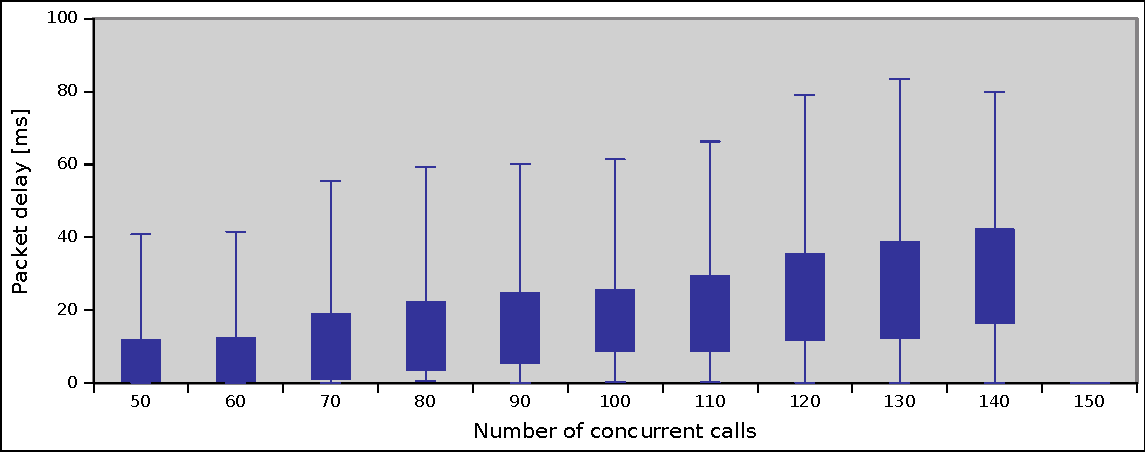
\includegraphics[width=15cm]{fig/serial-res.pdf}
\caption[Packet delay using serial implementation]{Visualization of distribution 
of delays during SRTP sessions with serial encryption implementation.}
\label{serial-res}
\end{figure}

Predictably the average delay of the packet increases with the amount of 
concurrent calls in figure \ref{serial-res} for serial implementation. The time
for 150 concurrent calls was not included due its excessive values which would
make readability of the graph more difficult. 

Even though the increase of delay seems to be linear, higher number of 
concurrent calls shows that the increase is exponential, which can be visible
on the figure \ref{pt-res} for persistent thread implementation.

\begin{figure}[H]
\centering
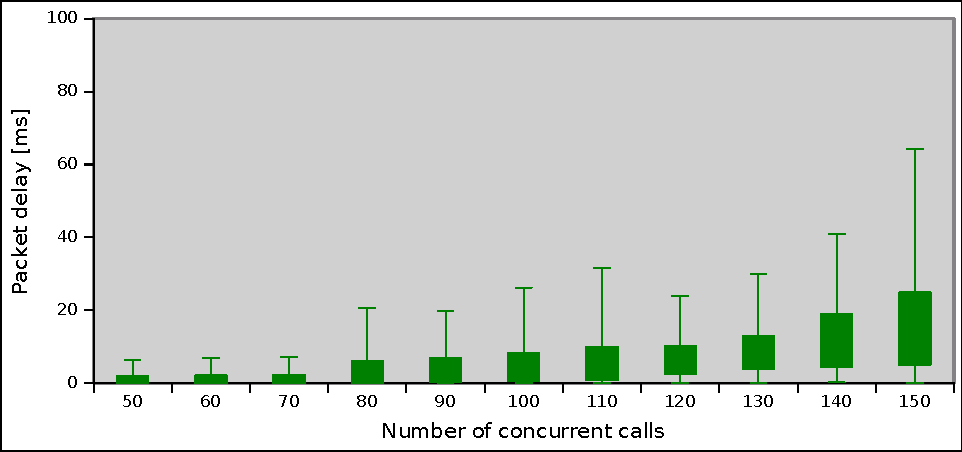
\includegraphics[width=15cm]{fig/persistent-thread-res.pdf}
\caption[Packet delay using parallel implementation]{Visualization of 
distribution of delays during SRTP sessions with parallel encryption 
implementation.}
\label{pt-res}
\end{figure}

Less predictable increase is visible in persistent thread implementation.
Inconsistent extreme values of delays may be produced by host and device
synchronization. Also memory management for packet buffer pool and OpenCL
buffer pool are two separate implementations, slowdown in one pool may have
negative effect on the other, therefore, both may combine in a negative way.

Comparing persistent thread implementation and serial implementation, the 
average delay was dropped to one half for smaller amount of concurrent calls
(50-90) and the best results of speed-up was achieved in 140 concurrent calls
where the average delay was dropped to one third.


\vspace{25em}
%\begin{figure}[H]
%\centering
%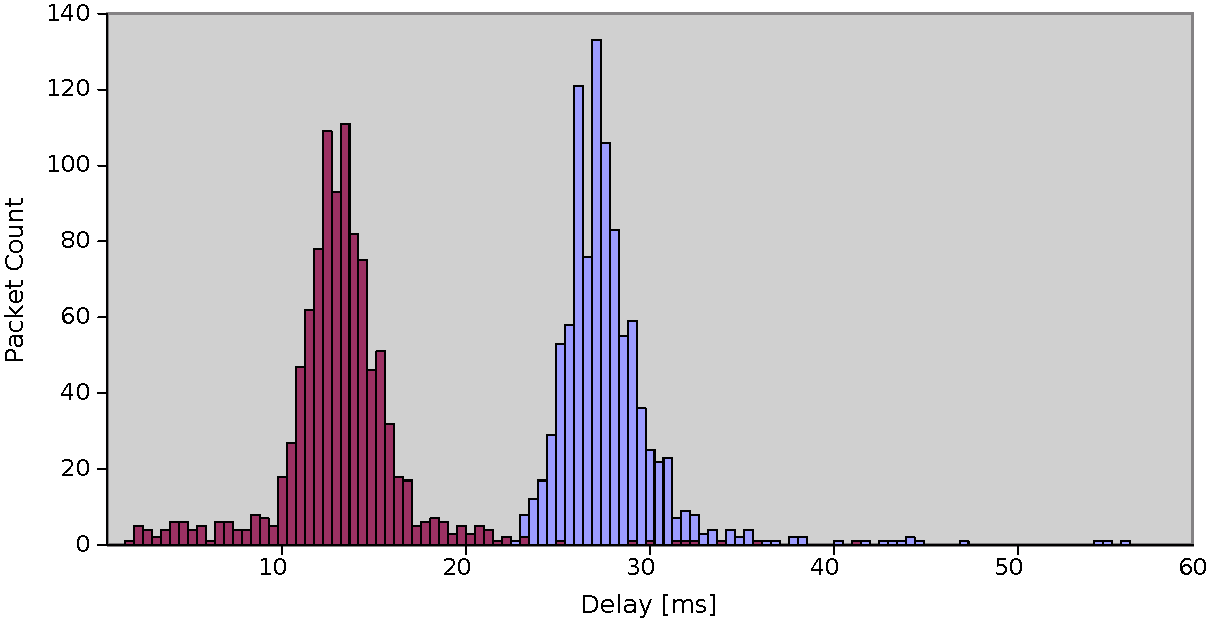
\includegraphics[width=15cm]{fig/delay_comparison.pdf}
%\caption[Comparison of packet delays]{Comparison of distribution of delays 
%during SRTP sessions serial with 
%parallel encryption implementation.}
%\label{dist-comp}
%\end{figure}  

The figure \ref{dist-comp} centralizes on the most interesting results from
previous tests which is the delay for 120 concurrent calls. The detailed 
distribution of packet delays shows, that parallel implementation, visualized
in blue color, has the peak situated around 12~ms when the serial 
implementation, visualized in purple color, has the most packet delays situated
around 27~ms.     



%%%%%%%%%%%%%%%%%%%%%%%%%%%%%%%%%%%%%%%%%%%%%%%%%%%%%%%%%%%%%%%%%%%%%%%%%%%%%%%%
\chapter{Conclusion}\label{chapter:conclusion}
There are lot of possibilities for optimization of SRTP processing. Selected
approach focuses on methods of parallelization of encryption and decryption
processes of default AES cipher, which offers large potential thanks to recent
development in the field of parallel computational units.

Proposed architectures and designs are currently far from being complete. The 
most effort was invested in correct analysis and understanding of basic 
principles of further implemented algorithms and elementary knowledge of 
parallel programming paradigm focused on usage of OpenCL framework for
general-purpose computations on graphical processing unit. Modern GPU 
concentrate large amount of computational power, which could be to a certain
extent utilized, if the algorithm is correctly mapped for parallel execution.
That brings unusual complications in design whose must be carefully considered.

Another important milestone is definition of integration of RTP stack with SRTP 
processing into implemented SIP Gateway and their mutual interaction. The SRTP 
processing is only a fraction of overall load on the gateway and if measured 
separately while producing exact experimental results may not be equal to the 
actual results on deployed machine experiencing real traffic. 

For the further development number of issues must be taken for notice. For 
instance the delay generated by the processing of separate SRTP packets should 
be reliably masked and interpolated across the SRTP stream to reduce possible 
jitter. On the other hand stands the actual delay of incoming packet, since
after certain absolute value the conversation quality becomes unbearable.

Nevertheless, partial value of this thesis lies in the understanding of current
technologies for future potential direction of development and exploration of
new options in the field communication infrastructure.



%=========================================================================
